%!TEX root = ../main.tex

\chapter{Experiment\label{chap:experiment}}

\section{Setup}

The experiment was performed with two X500 \ac{UAV}s, each of them equipped with a Prophesee EVK4 event-based camera, one with a 2.5mm f/1.6
fish eye lens with an \ac{FOV} of roughly 187 degrees and the second one with Entaniya 1.07mm f/2.8 fish eye lens with an \ac{FOV} of 280 degrees.
Each UAV is also equipped with a Basler camera with a fish eye lens, to provide normal video signal that is recorded alongside the event stream
from the event-based camera.
Both cameras are connected to the onboard Intel NUC computer running the ROS system, on which all the processing is done during the flight. Both 
\ac{UAV}s are also equipped with a \ac{RTK} module, which is used to localize the \ac{UAV}, and is used as ground truth data for the pose estimation.
The UVDAR blinking frequencies $\mathcal{F} = \{4.0, 2.0, 1.\overline{3}, 1.0\}$ (in kHz) were defined, where each of the arms were blinking at its assigned
frequency.
The measurements were collected during the \ac{MRS} Camp in Temešvár in August 2025, the \ac{UAV}s can be seen on \reffig{fig:uav33_37}.
\begin{figure}[H]
	\centering
	\subfloat[UAV33] {
	  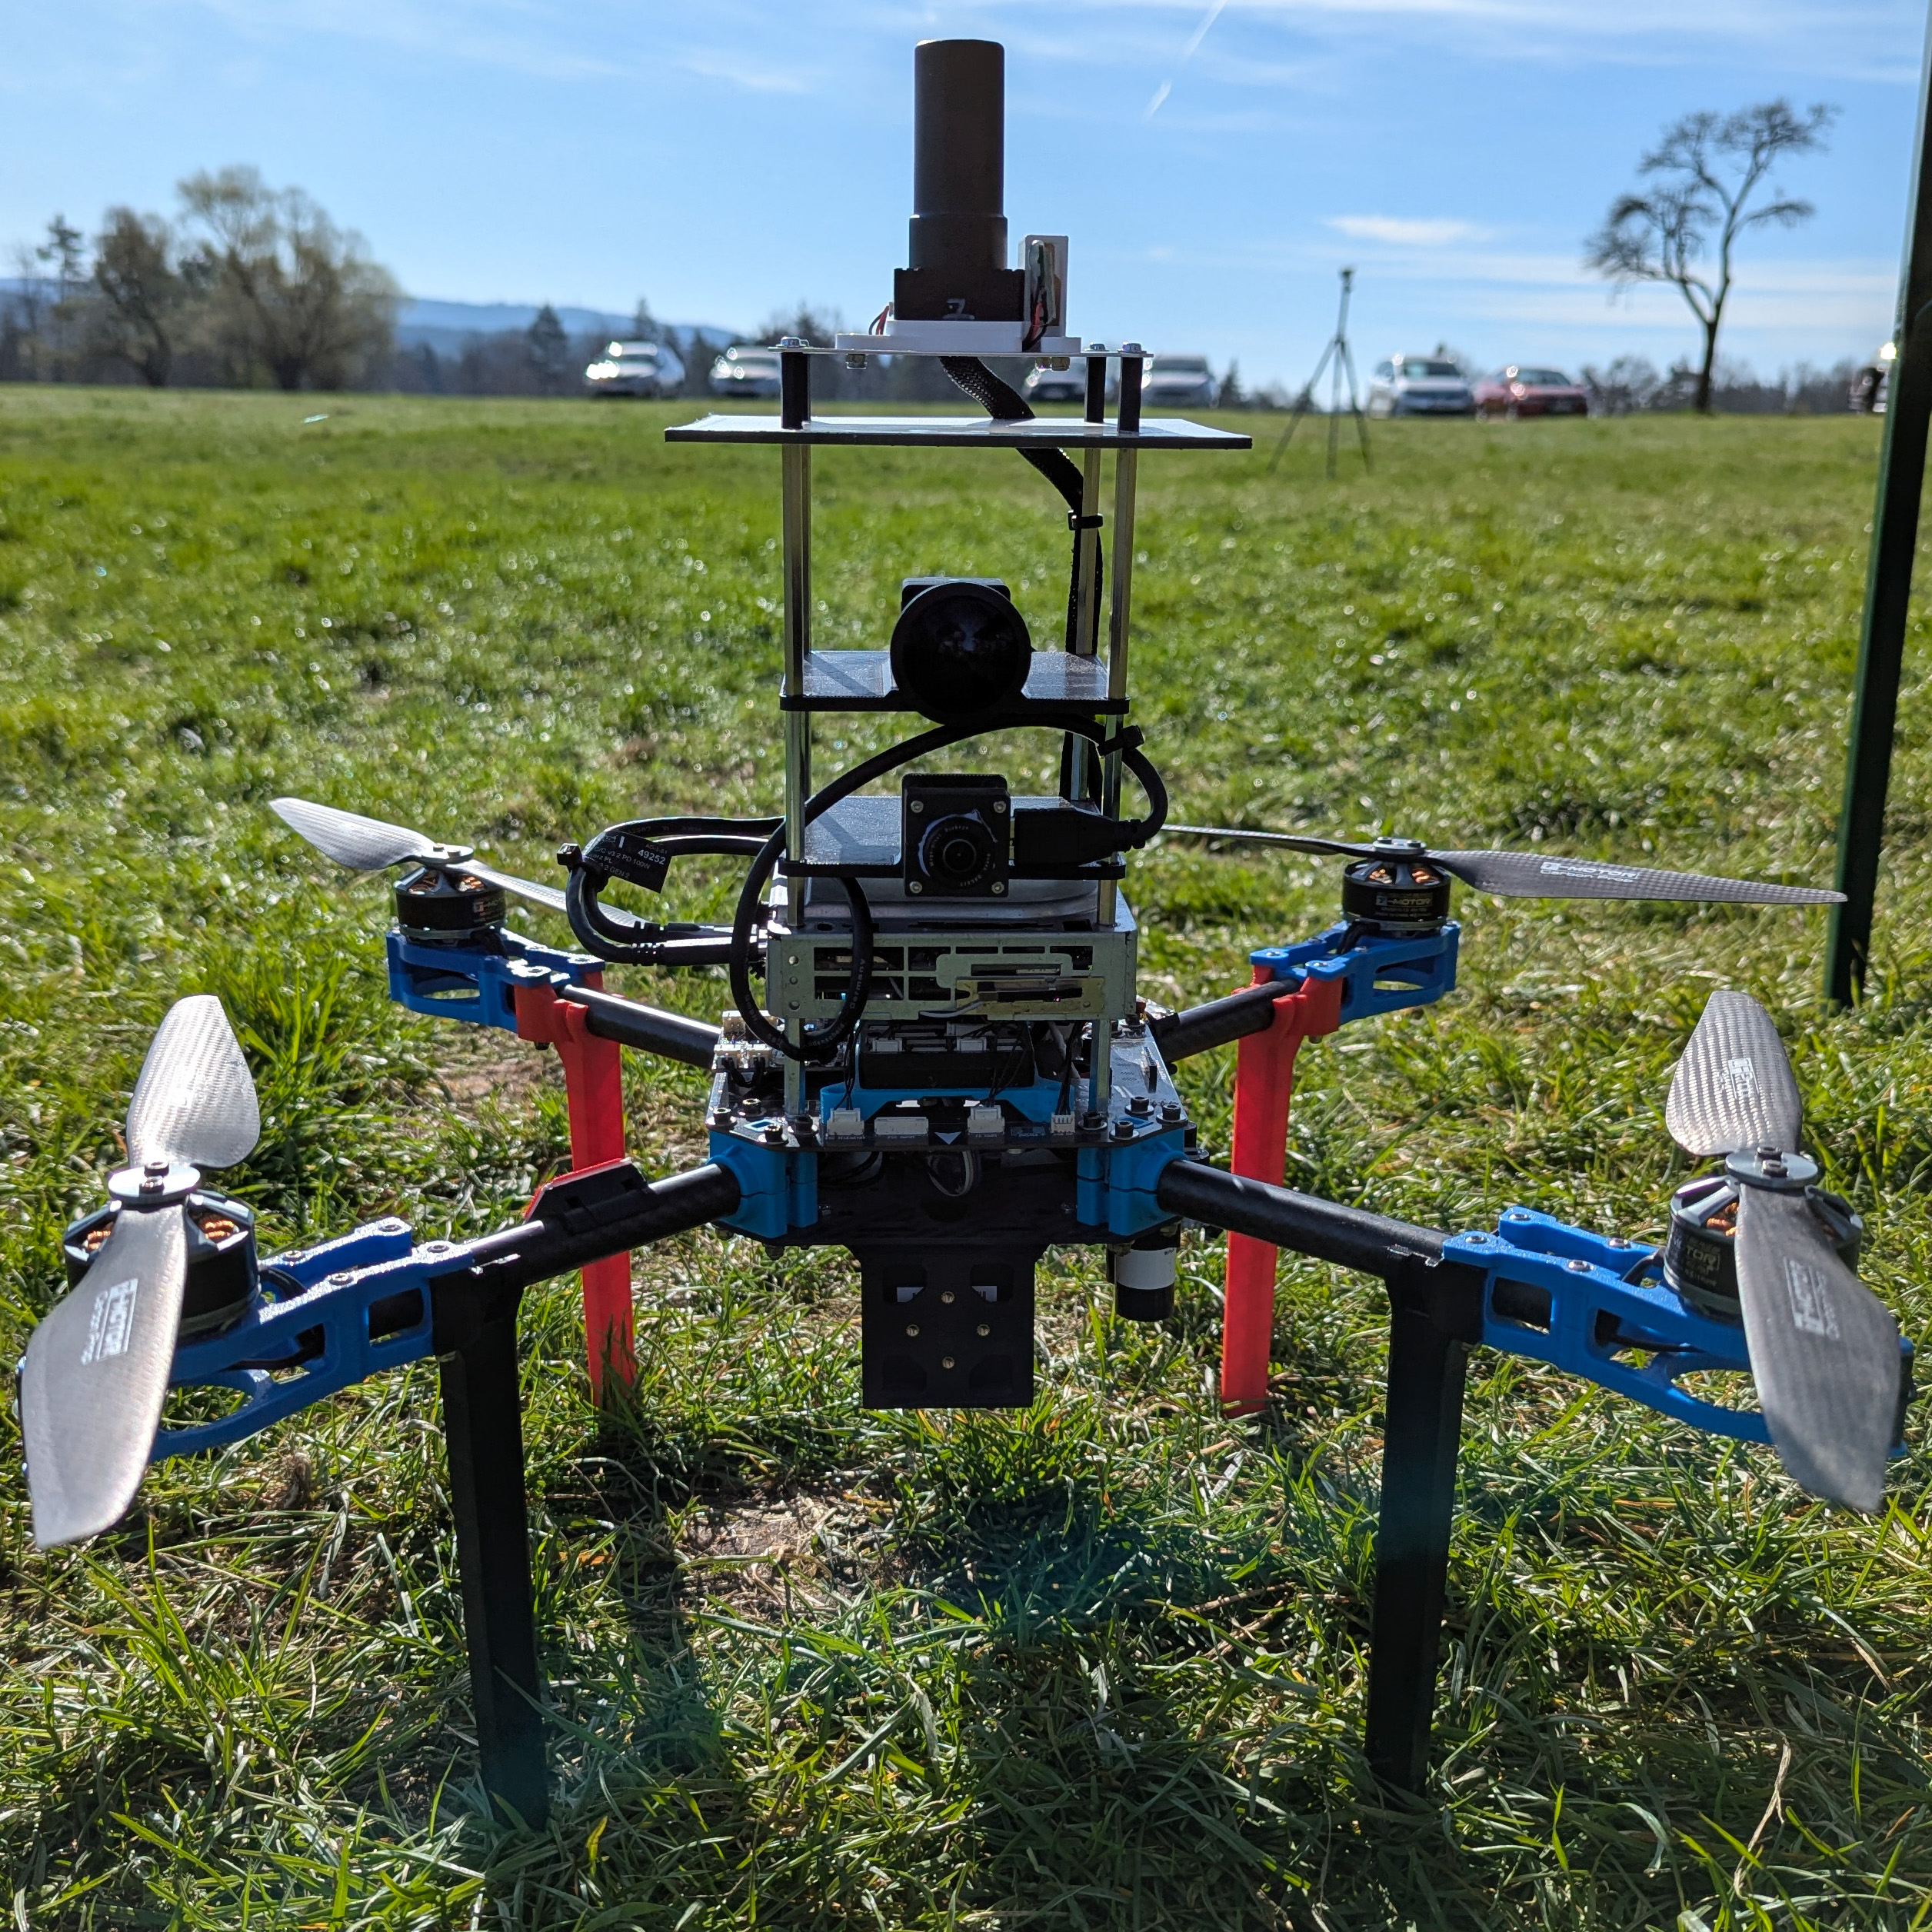
\includegraphics[width=0.4\textwidth]{./fig/photos/uav33.jpg}
	  \label{fig:uav33}
	}
	\subfloat[UAV37] {
	  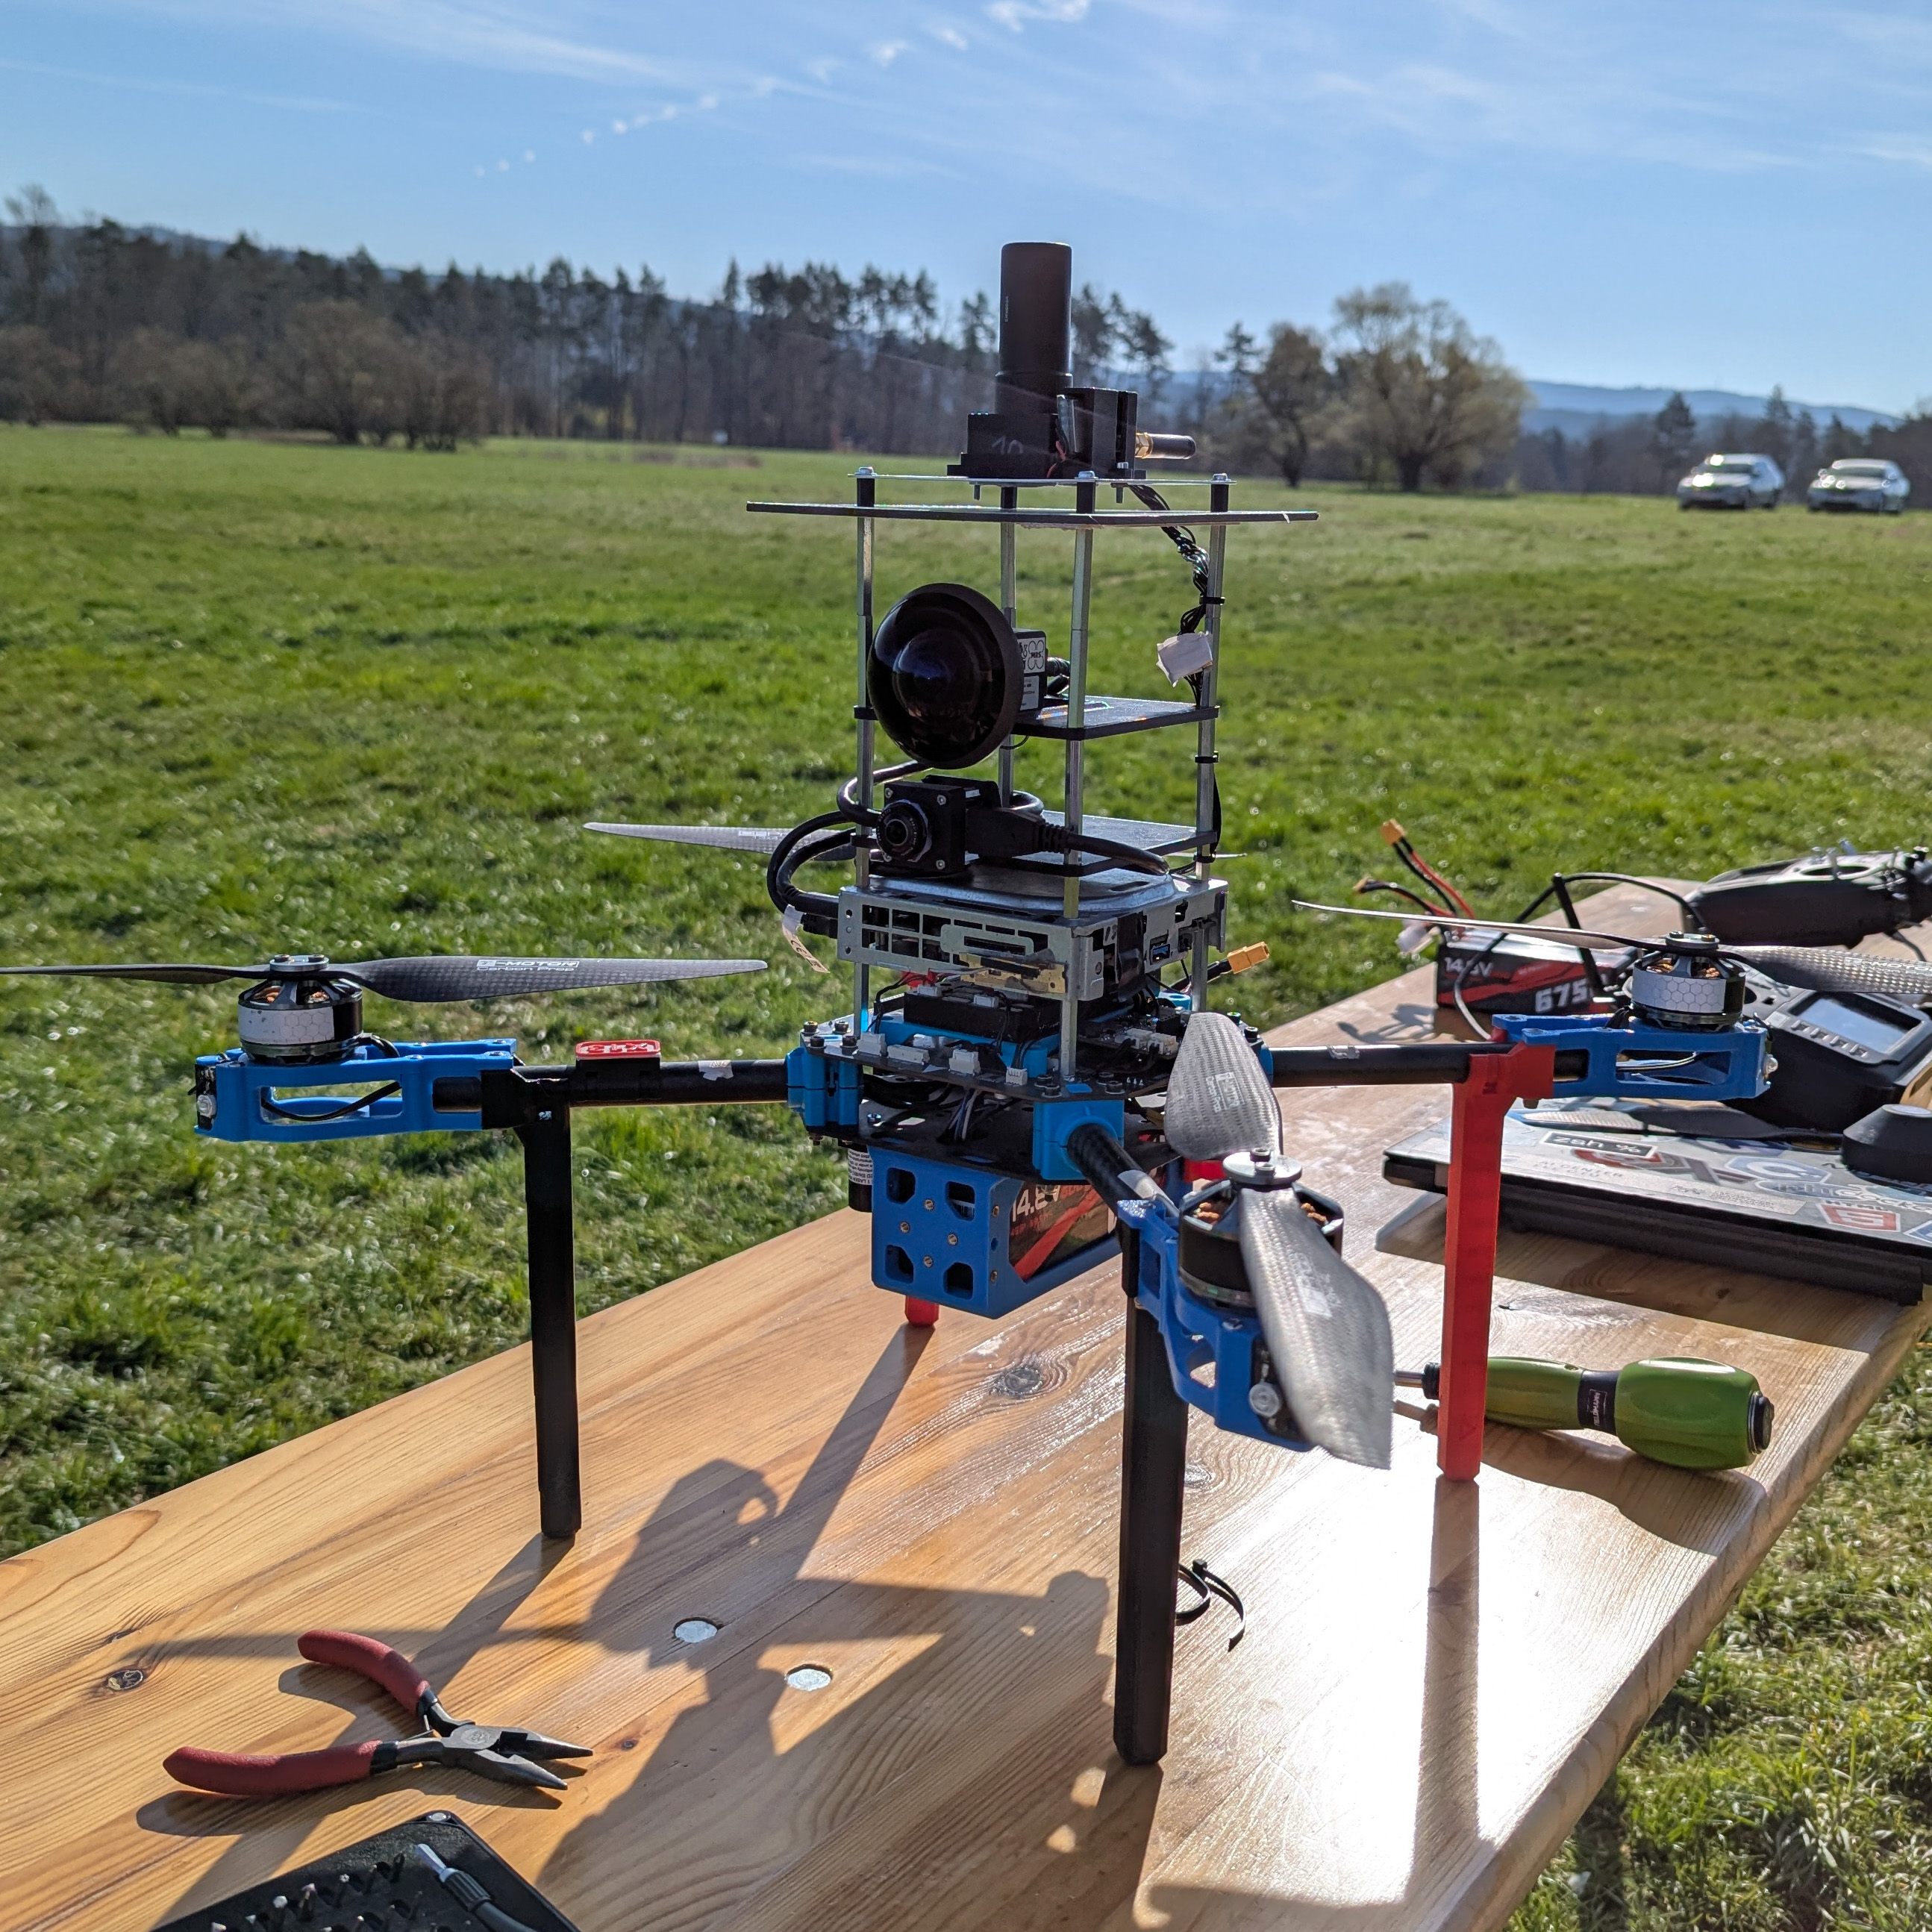
\includegraphics[width=0.4\textwidth]{./fig/photos/uav37.jpg}
	  \label{fig:uav37}
	}
	\caption{
		Two X500 UAVs, UAV33 on \reffig{fig:uav33} and UAV37 on \reffig{fig:uav37}.
  }
	\label{fig:uav33_37}
\end{figure}
Two pilots manually controlled the \ac{UAV}s, systematically varying the distance and angles between them to generate diverse measurement data during the experiment. All in-flight data, including sensor measurements and camera streams, we recorden in a \ac{ROS} bag file for subsequent analysis
in a simulated environment. In addition, raw event stream data from the event-based camera was also recorded and saved. The camera view from the UAV33
can be seen on \reffig{fig:exp1}. During the recording about $17$ million events were generated every second by each camera, which equates to a data
throughput of about $45$ MB per second per drone. Each raw recording is about $14$ gigabytes in size.

\begin{figure}[H]
	\centering
	\subfloat[Event-based camera output] {
	  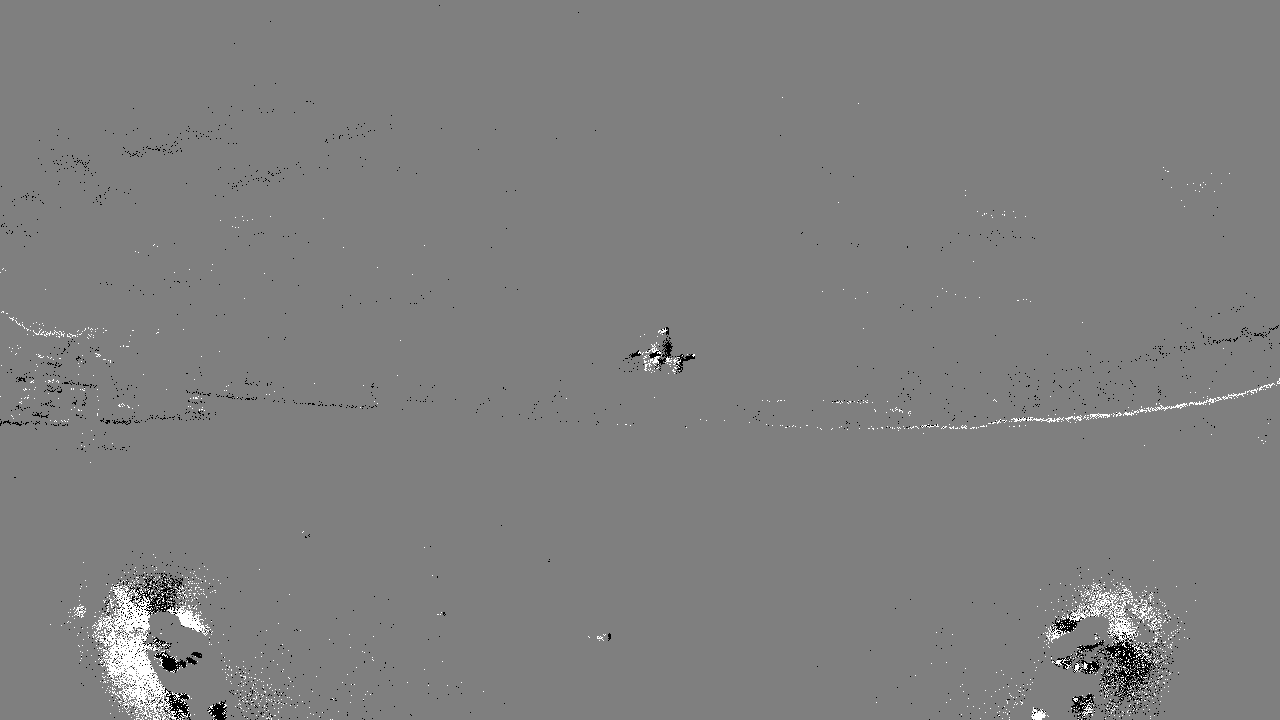
\includegraphics[width=0.50\textwidth]{./fig/photos/uav33_event.png}
	  \label{fig:exp1_event}
	}
	\subfloat[Basler camera output] {
	  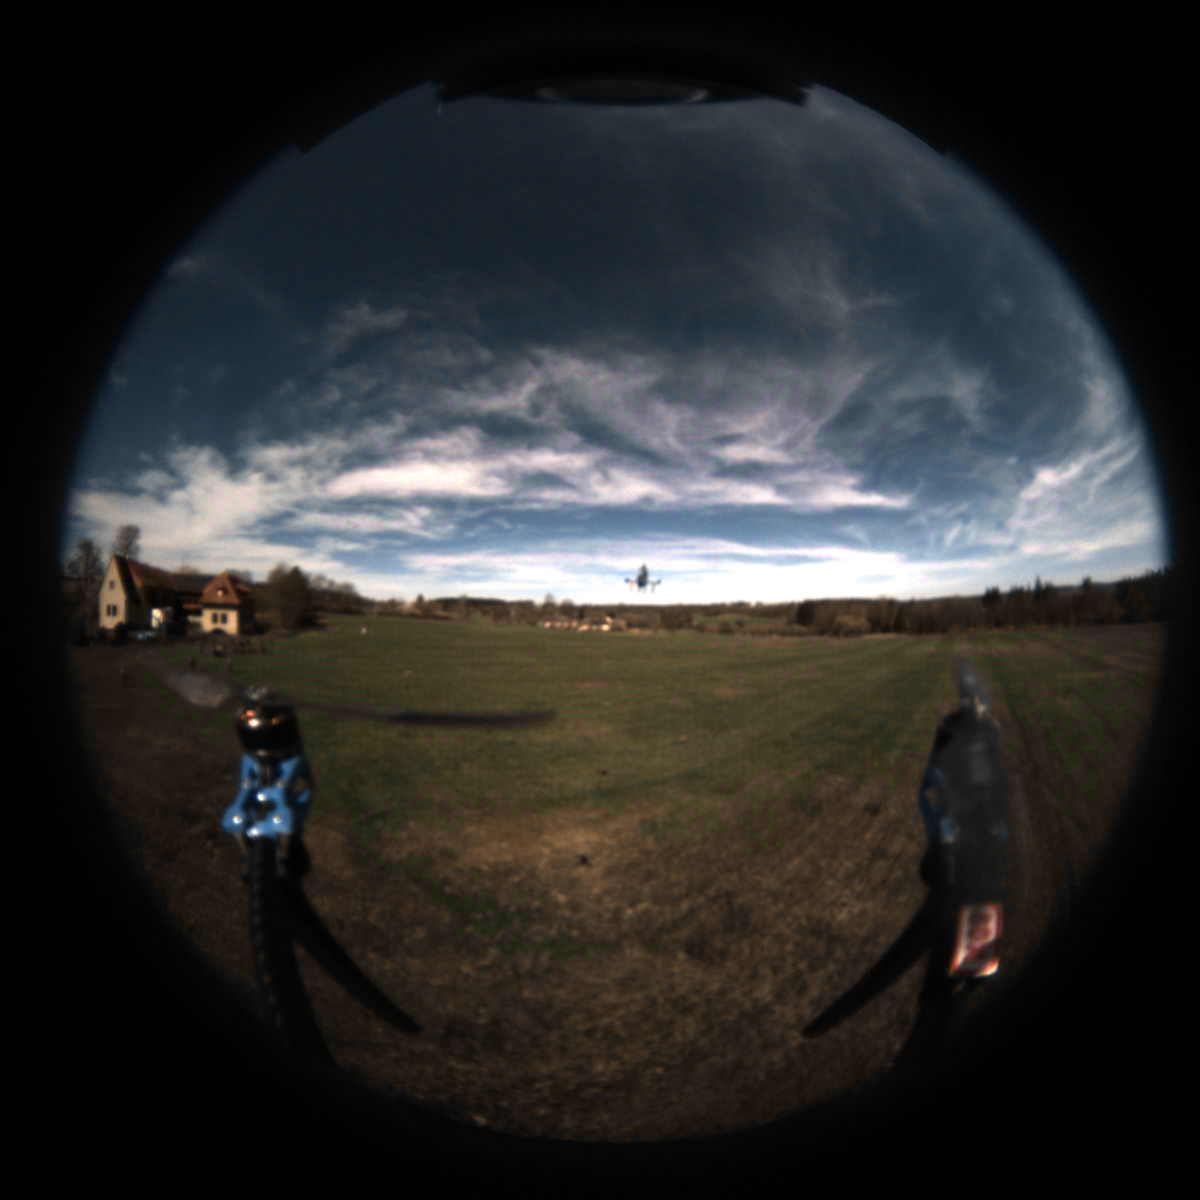
\includegraphics[width=0.282\textwidth]{./fig/photos/uav33_basler.png}
	  \label{fig:exp1_basler}
	}
	\caption{
		The view of the experiment from UAV33, with event data on \reffig{fig:exp1_event} and Basler camera view on \reffig{fig:exp1_basler}.
  }
	\label{fig:exp1}
\end{figure}

%\todo{SHOW MEASURED DATA FROM RQT}

%\todo{SHOW GNSS/ESTIMATION DIFFERENCES}

%\todo{SHOW THE RVIZ/RQTPLOT VISUALIZATION PIPELINE}

\section{Analysis}

The data was analyzed after the recording, by generating image frames from the raw event recordings. This data,
as seen on \reffig{fig:labeled}, has then been manually labeled and with the use of a blob detector the \ac{LED} sources
were selected.
\todo{maybe write more}

\begin{figure}[H]
	\centering
	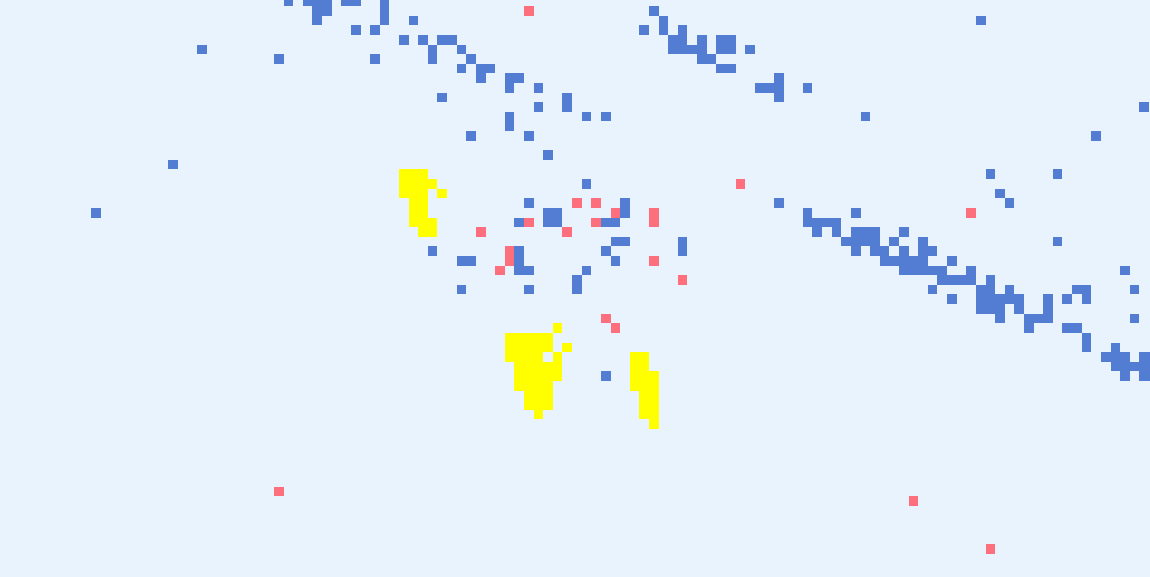
\includegraphics[width=0.7\textwidth]{./fig/photos/labeled_2.png}
	\caption{Labeled blob centers}
	\label{fig:labeled}
\end{figure}

\section{Experiment results}

For each labeled group of points a distance estimation was performed using the \texttt{DistanceEstimator} using the
\ac{P3P} algorithm. For each estimated pose, a distance from the camera was calculated, which was then compared to the
ground truth distance obtained from the \ac{GNSS}. The distance is calculated as a norm of the difference of the \ac{UAV} positions.
The results demostrate, that our approach achieves a mean absolute error of $2.47$ meters, with a standard deviation of $1.75$ meters,
indicating moderate precision under the experiment conditions.
The estimation
results can be seen on \reffig{fig:experiment_results}

\begin{figure}[H]
	\centering
	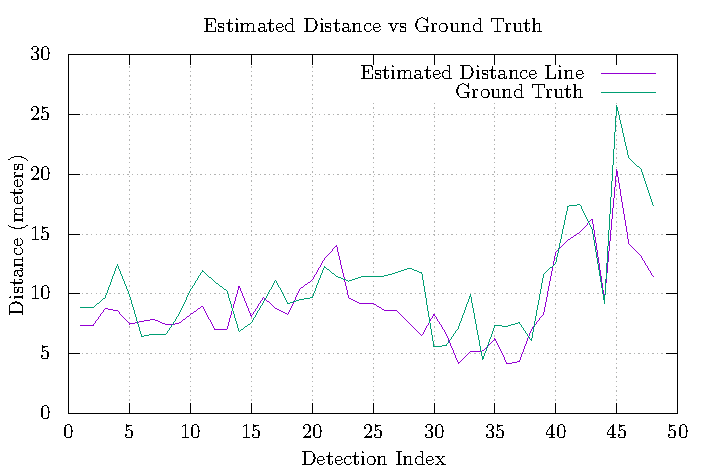
\includegraphics[width=0.7\textwidth]{./fig/tikz/experiment_analysis.pdf}
	\caption{The distance estimation data from the experiment, compared with the recorded GNSS data used as ground truth}
	\label{fig:experiment_results}
\end{figure}

\section{Real life deployment - estimation challenges}

The analysis presents several challenges, one of them being the identification of the moving \ac{UAV} in the recorded
data. The ideal solution is to identify which pixels are being generated with their specific frequeny, which the \ac{LED}
markers are set to blink on the. Sadly, during the measurement of our experiment, the \ac{UAV} produced a lot
of vibration in the data, which interfered with our measurements, and thus the detection of blobs has become a large obsacle.
When we generate images from the recording, the problem persists; How do we identify the correct blobs automatically, when
the \ac{UAV} can be at an arbitrary distance and orientation?
Manual labeling is not the definitive answer to our problem either because even the blob center selection itself can greatly
influence the estimation precision. In \reffig{fig:blob_comb}, we select a single pixel from each blob and run the distance estimation
for each combination of pixel. As we can observe, even a change in the range of 3 pixels can change the estimated distance by
$1.5$ meters. The center of a blob may be calculated as a geometrical center of the blob's pixels, but this approach fails
when the blob contains pixels which do not belong to them.
%Secondly, the calculation of the exact center would most likely yield results with sub-pixel level precision, requiring the placement of the center between the pixels

%As we have shown in \reffig{fig:labeled}, there exist a challenge of \ac{UAV} identification 
\begin{figure}[H]
	\centering
	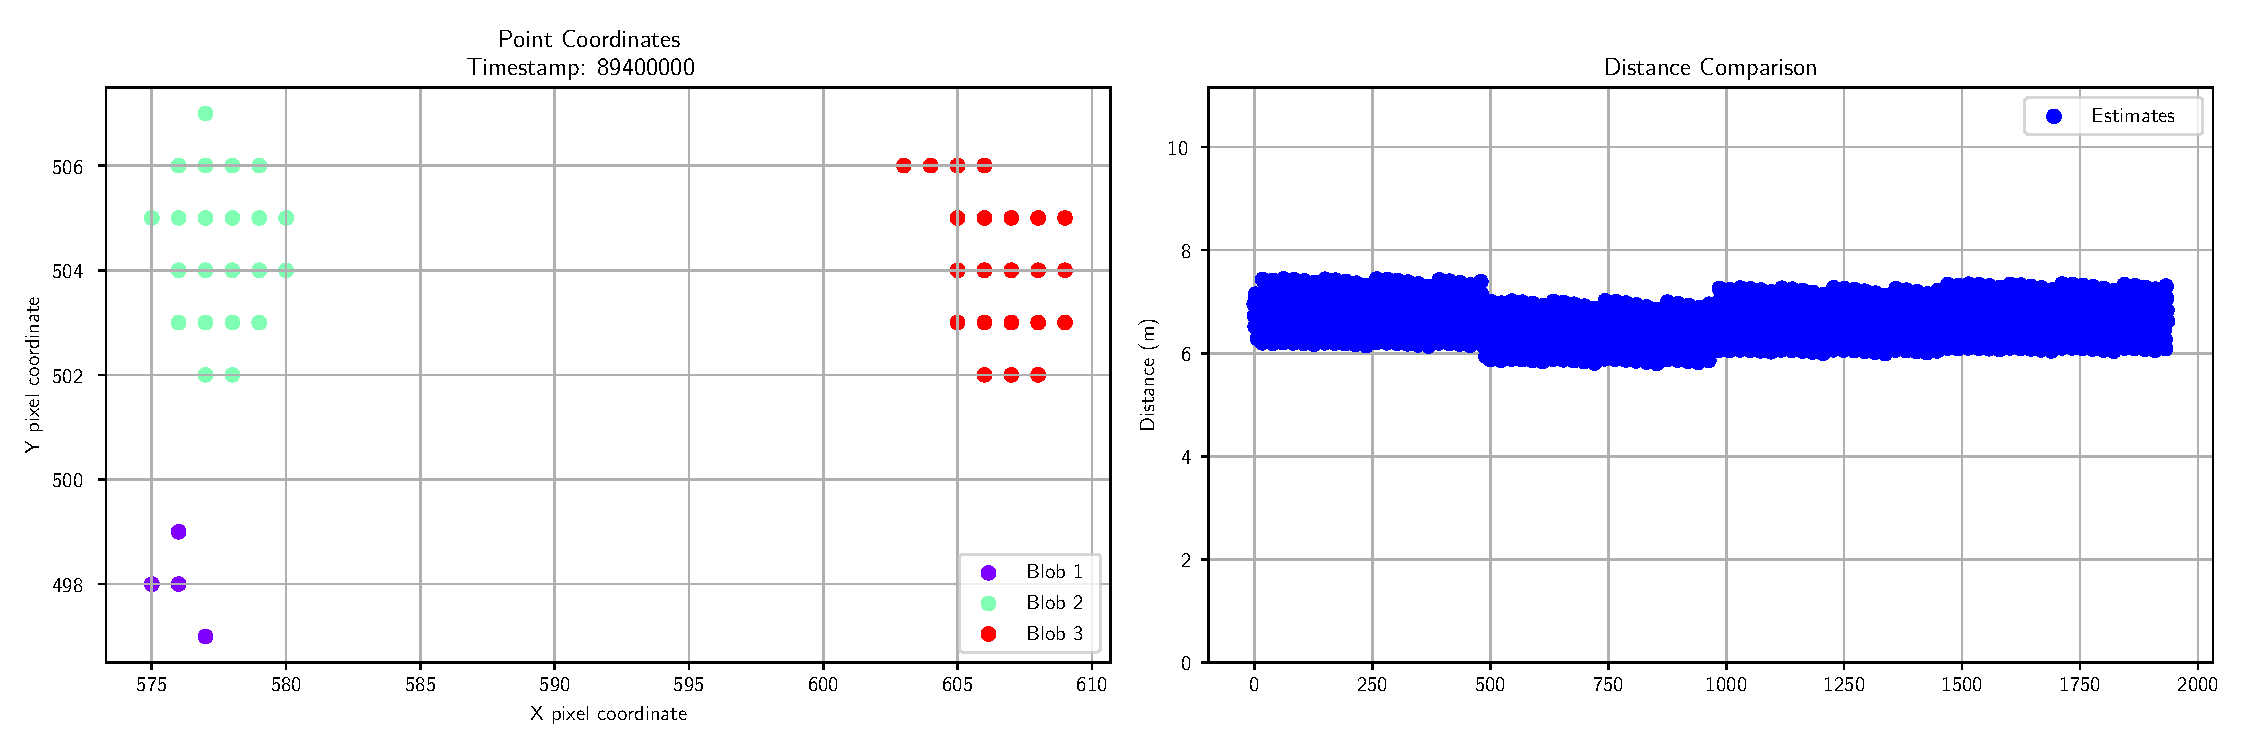
\includegraphics[width=0.99\textwidth]{./fig/pgfplot/estimation_selection_1.pdf}
	\caption{Blob centers with the resulting distance estimations for any combination of center selection}
	\label{fig:blob_comb}
\end{figure}

A fundamental limitation of any vision‐based positioning system is the finite spatial resolution of the camera sensor. As the distance to the \ac{LED}s increases, beyond roughly $20$ m in our setup, their angular size on the image plane decreases to just a few pixels. Once a marker spans only a few sensor pixels, adjacent light sources can begin to merge: individual \ac{LED} spots can no longer be differentiated and their point-spread functions overlap. This blending of pixel responses prevents the reliable separation of each \ac{LED} signal and ultimately makes accurate detection and decoding impossible.